\documentclass[10pt]{article}
\setlength{\parindent}{0cm}
\usepackage{amsmath, amssymb, algorithm, algorithmic, graphicx, cancel}
\usepackage{tikz}
\title{sphere points notes}
\date{}
\author{arvind rao}

\begin{document}
\maketitle

\section*{Seed The Sphere}
We seed the sphere $S^2 \subset \mathbb{R}^3$ with points drawn from the uniform distribution, on the sphere. Do do this, we need the probability mass function of the sphere, which is: $d \mu = \frac{1}{4 \pi}\sin(\theta) d \theta d\varphi$ in $\theta, \varphi$ coordinates.  

\[
 		\int_{S^2} d \mu = \int^{2\pi}_{0} \int^{\pi}_{0} \frac{1}{4\pi}\sin(\theta) d \theta d\varphi = 1
\]

Working in $\theta, \varphi$ coordinates, our goal is to generate $\theta, \varphi$ so that they are equally likely. The joint cdf is:

\begin{align*}
	F(\theta, \varphi)  & = \int^{\varphi}_{0} \int^{\theta}_{0} \frac{1}{4\pi}\sin(\tilde{\theta}) d \tilde{\theta} d\tilde{\varphi} \\
								 & = \frac{1}{4\pi} \varphi (1 - \cos(\theta))
\end{align*}

Its clear from definition of the join cumulative distribution ( and the p.d.f) that $\theta$ and $\varphi$ are independent.

\[
	F(\theta, \varphi) = \frac{\varphi}{2\pi} \frac{1 - \cos(\theta)}{2}
\]

Which yields two c.d.fs:
\[
	F_{\varphi}(\varphi) = \frac{\varphi}{2\pi} \quad \text{and} \quad F_{\theta}(\theta) = \frac{1 - \cos(\theta)}{2}
\]

Furthermore,

\[
			P( x < \varphi ) = F_{\varphi} \quad \text{and} \quad P( y < \theta ) = F_{\theta} 
\]

Then generating probabilities and solving for $\theta$ and $\varphi$ will yield an equally likely pair. In brief here is the algorithm:

\begin{algorithm}
\caption{Uniformly Generate $(\theta, \varphi) \in S^2$ }
\begin{algorithmic} 
\STATE Draw $X \thicksim U([0,1])$ and $Y \thicksim U([0,1])$
\STATE set $\theta = F_{\theta}^{-1}(X)$
\STATE set $\varphi = F_{\varphi}^{-1}(Y)$

\RETURN $\theta$ and $\varphi$        
\end{algorithmic}
\end{algorithm}

\section*{Gradient Descent Method For Finding Optimal Point Configuration}

For low number point configurations \textit{e.g.} $2, 3$, etc. we can output a memorized solution. For high $N$ this won't work, because such configurations are not necessarily know or easy to derive, hence this project. The novelty of the proposed method is to take into account the intrinsic geometry of $S^2$. The plan is sample the uniform distribution of the sphere, drawing $N$ points, and then simulate electrostatic repulsion on the sphere. The main differences between simulation in plane and $S^2$ are distance functions and projection from the tangent plane back to the base space. In both cases Columb energy is

\[
		E(p,q) = \frac{1}{d(p,q)}
\]

Here $d(p,q)$ is the distance between points $p$ and $q$. The spherical distance for $p, q \in S^2 \subset \mathbb{R}^3$ is $\arccos(p \cdot q)$. So on the sphere the electro-static force between points is:

\[
	E(p,q) = \frac{1}{\arccos(p \cdot q)}
\]

Alternatively, one could investigate configurations which minimize energies in the family:
\[
		E(p,q) = \Big( \frac{1}{\arccos(p \cdot q)}  \Big)^s \quad \text{ for } s= 1, \ldots, N
\]

Fix $p \in S^2$ and define $E_p(x) = E(p,x)$. The gradient flow of a single point is 
\[
	\frac{dx(t)}{dt} = - \nabla E_p(x)
\]


The flow is on $x$, in particular we think of $x$ as reacting to $p$. What's the gradient?  Further, let $x = (\cos(\varphi) \sin(\theta), \sin(\varphi)\sin(\theta), \cos(\theta))$. From which we know that:

\[
\nabla x = 
\left[
	\begin{array}{cc}
		cos(\varphi) \cos(\theta) & -\sin(\varphi) \sin(\theta) \\
		  \sin(\varphi)\cos(\theta) & \cos(\varphi)\sin(\theta)  \\
		-\sin(\theta) & 0 
	\end{array}
	\right]
\]

\begin{align*}
	\nabla E_{x}(s) &= - \Big( \frac{1}{\arccos(s \cdot x)} \Big)^2 \nabla_s \arccos(s \cdot x) \\
						  &=  \Big( \frac{1}{\arccos(s \cdot x)} \Big)^2 \frac{1}{\sqrt{1 -  (s \cdot x)^2 }} \nabla_s (s \cdot x)\\
						  &=  E_{x}(s)^{2} \frac{1}{\sqrt{1 -  (s \cdot x)^2 }}
\left[
\begin{array}{ccc}
x_1, x_2, x_3
\end{array}
\right]
\left[
	\begin{array}{cc}
		cos(\varphi) \cos(\theta) & -\sin(\varphi) \sin(\theta) \\
		  \sin(\varphi)\cos(\theta) & \cos(\varphi)\sin(\theta)  \\
		-\sin(\theta) & 0 
	\end{array}
	\right]
\end{align*}

The tangent plane at $s \in S^2$ is spanned $s_{\theta} = 	\left[\begin{array}{cc}
		cos(\varphi) \cos(\theta)  \\
		  \sin(\varphi)\cos(\theta)  \\
		-\sin(\theta)  
	\end{array}\right]$
and $ s_{\varphi} = \left[
	\begin{array}{cc}
		-\sin(\varphi) \sin(\theta) \\
		  \cos(\varphi)\sin(\theta)  \\
		 0 
	\end{array}
	\right]$.

So then the intrinsic form of $\nabla E$ is:
\begin{align*}
\nabla_{s} E_{x}(s)  &=  E(s, x)^{2} \frac{(x \cdot s_{\theta}) s_{\theta} + (x \cdot s_{\varphi}) s_{\varphi}}{\sqrt{ 1 -  (s \cdot x)^2 }} 
\end{align*}

Because of compactness, $x$ acts on $s$ from two directions on the great circle connecting them.

\[
		D(p,q) = \frac{1}{2\pi - \arccos(p \cdot q)}
\]

 The other force is:
\[
\nabla_{s} D_{x}(s) =  - D(s, x)^{2} \frac{(x \cdot s_{\theta}) s_{\theta} + (x \cdot s_{\varphi}) s_{\varphi}}{\sqrt{1 - (s \cdot x)^2 }} 
\]

The combined ( or total ) influence of $x$ on $s$ is:
\[
	\nabla_s E_x(s)  - \nabla_{s} D_{x}(s) = \Big(D(s, x)^{2} - E(s, x)^{2} \Big) \frac{1}{\sqrt{1 -  (s \cdot x)^2 }} \Big( (x \cdot s_{\theta}) s_{\theta} + (x \cdot s_{\varphi}) s_{\varphi} \Big)
\]
 
Notationally, $\nabla_x$ is the derivative in $x$. And

\[
	\nabla_s E_x(s) |_{s=p} \in T_{p}S^2.
\]

Let $\mathcal{A} = \{ x_1, \ldots, x_N \}$ be the sampled sphere points, and $p \in \mathcal{A}$.

\begin{figure}
	\centering
	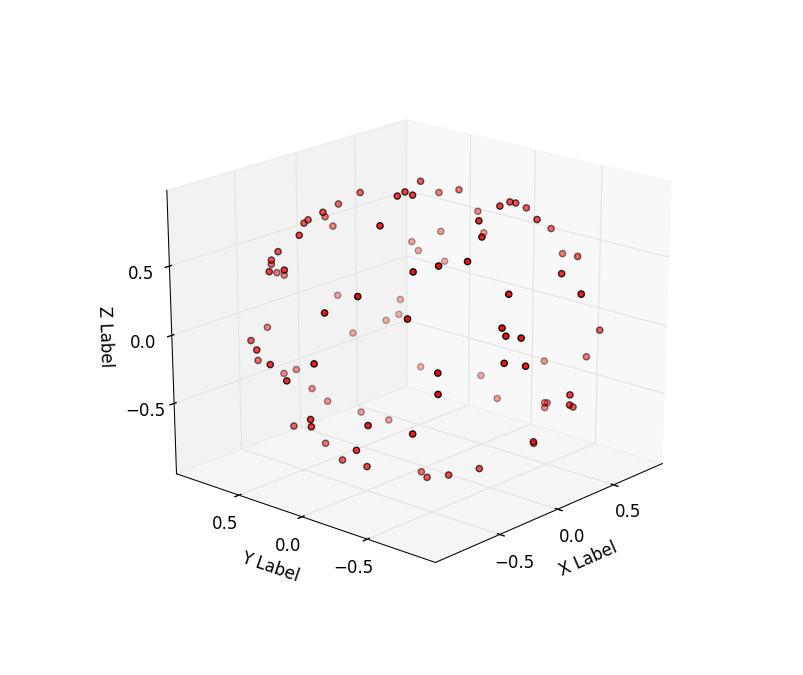
\includegraphics[scale=0.5]{uniform_sphere_points.png}
	\caption{$N=100$ point sampled from the uniform distribution on the sphere.}
	\label{fig:sampledpoints}
\end{figure}

From Figure \ref{fig:sampledpoints} it's clear the sampled points are far from an equal distance configuration--our goal. The algorithm for moving points to the desired configuration, proceeds by computing the combined electrostatic force exerted on each individual of the points the collection. Taking each point $p \in \mathcal{A}$ as a reference point. One computes the combined effect of all the other points on $p$.

\[
	\sum_{x \in \mathcal{A}} \nabla_s E_x(s)  - \nabla_{s} D_{x}(s) |_{s=p}  \in T_{p}S^2.
\]

Suppose $p_n$ is the $n$th iteration of $p \in \mathcal{A}$. Then according to the discrete flow in euclidean space would be:

\begin{equation}
p_{n+1} - p_{n} = - \Delta t \cdot \sum_{x \in \mathcal{A}} \nabla_s E_x(s) - \nabla_{s} D_{x}(s) |_{s=p_n} 
\end{equation}

However, we aren't working in euclidean space. There's no canonical identification of tangent vectors with points on $S^2$. But we have the exponential map, which does take vectors to points in the underlying space; and we will use mapping to give our next point. With all this in mind, the discrete flow on $S^2$ is:

\[
	p_{n+1} = exp_{p_{n}}\Big( - \Delta t \cdot \sum_{x \in \mathcal{A}} \nabla_s E_x(s) - \nabla_{s} D_{x}(s) |_{s=p_n} \Big)
\]


Compute the hessian of $E_x(s)$. Start by computing the $s_{\theta \theta}$, $s_{\varphi\varphi}$, and $s_{\theta \varphi}$.

\begin{gather*}
s_{\theta \varphi} = ( -\sin(\varphi) \cos(\theta), \cos(\varphi)\cos(\theta), 0 ) \\
s_{\theta \theta} = (-\cos(\varphi) \sin(\theta), -\sin(\varphi)\sin(\theta), -\cos(\theta)) \\
s_{\varphi \varphi} = (-\cos(\varphi) \sin(\theta), -\sin(\varphi)\sin(\theta), 0)
\end{gather*}

\begin{gather*}
s_{\theta \varphi} \cdot s_{\theta} = 0 \\
s_{\theta \varphi} \cdot s_{\varphi} = \frac{1}{2} \sin(2\theta)\\
s_{\theta \theta} \cdot s_{\theta} =  0 \\
s_{\theta \theta} \cdot s_{\varphi} =  0\\
s_{\varphi \varphi} \cdot s_{\theta} = -\frac{1}{2} \sin(2\theta) \\
s_{\varphi \varphi} \cdot s_{\varphi} = 0 
\end{gather*}

\begin{align*}
\nabla^2 f &= f_{\theta \theta} s_{\theta} + \cancelto{0}{f_{\theta} s_{\theta \theta}} + f_{\theta \varphi} s_{\varphi} + f_{\varphi} s_{\varphi \theta} + f_{\theta \varphi} s_{\theta}  + f_{\theta} s_{\theta \varphi} + f_{\varphi \varphi} s_{\varphi} + f_{\varphi} s_{\varphi \varphi} \\
	&= f_{\theta \theta} s_{\theta} + f_{\theta \varphi} s_{\varphi} + f_{\varphi} \frac{1}{2} \sin(2\theta) s_{\varphi} +  f_{\theta \varphi} s_{\theta} + f_{\theta} \frac{1}{2} \sin(2\theta) s_{\varphi} + f_{\varphi \varphi} s_{\varphi} - f_{\varphi} \frac{1}{2} \sin(2\theta) s_{\theta}\\
	&= f_{\theta \theta} s_{\theta} +  f_{\theta \varphi} s_{\theta} - f_{\varphi} \frac{1}{2} \sin(2\theta) s_{\theta} + f_{\theta \varphi} s_{\varphi} + f_{\varphi} \frac{1}{2} \sin(2\theta) s_{\varphi} + f_{\theta} \frac{1}{2} \sin(2\theta) s_{\varphi} + f_{\varphi \varphi} s_{\varphi} \\
	&=  \Big[ f_{\theta \theta} +  f_{\theta \varphi} - f_{\varphi} \frac{1}{2} \sin(2\theta) \Big] s_{\theta} + \Big[ f_{\theta \varphi} + f_{\varphi} \frac{1}{2} \sin(2\theta) + f_{\theta} \frac{1}{2} \sin(2\theta) + f_{\varphi \varphi} \Big] s_{\varphi} 
\end{align*}


%\begin{algorithm}
%\caption{Compute the direction to move one point from $\mathcal{A}$}
%\begin{algorithmic} 
%\STATE choose $p \in \mathcal{A}$, and define $\tilde{\mathcal{A}}$ to be $\mathcal{A} - \{p\}$
%\LOOP $x \in \tilde{\mathcal{A}}$
%\ENDLOOP
%%\STATE
%%\RETURN      
%\end{algorithmic}
%\end{algorithm}



\end{document}